\subsection{Transformers and pre-trained language models for finance}

% 
% Version: 2.5.3
% Last updated: 2026-07-21
% Provenance: third chapter of Part V of the 2nd edition, extracted from the
% monolithic Chapter_20_Draft19.md (v3.9.7, archived in
% `_archive_monolithic_v3.9.7/`).
%

\subsubsection{Introduction}

The embeddings of Chapter 21 lift bag-of-words representations into a dense, distributional space, but they remain \textit{context-blind}: every word has exactly one vector regardless of the surrounding sentence. For financial text this is a binding limitation. \textit{Volatility} in an options-pricing discussion sits in a different region of the language space than \textit{volatility} in a political-stability discussion; \textit{exposure} across market risk, media attention, and environmental contamination should occupy three different points, not one. Resolving this limitation requires an architecture in which a token's representation depends on the entire input sequence rather than on the token's type alone.

The transformer architecture introduced by \cite{vaswani2017attention} provides exactly that. Each token is encoded conditional on every other token in the sequence through a self-attention mechanism, and stacking such layers produces representations in which \textit{the} contextual encoder is the model rather than a fixed table. We develop the architecture from first principles, cover the transfer-learning paradigm that has made pre-trained language models practical, and survey the finance-specific pre-trained models built on it. The decoder-only and encoder-decoder variants that underpin large language models are introduced here, but their full treatment is deferred to Chapter 23.

The methodological progression of this chapter parallels the architectural progression of the field between 2017 and 2020: attention as a generic mechanism (2017), BERT as the canonical pre-trained encoder (2018), and finance-specific pre-trained models (2019 onward).

\subsubsection{Why attention changed everything}

The classical methods of Chapter 20 represent text as a bag of words, and the embeddings of Chapter 21 as static vectors, both discarding the sequential structure of language. Recurrent neural networks (RNNs) and their variant, long short-term memory networks (LSTMs) introduced by \cite{hochreiter1997long}, addressed this by processing text sequentially, maintaining a hidden state that evolves as each word is read (see Chapter 7 for neural network foundations). Concretely, the LSTM cell at position $t$ takes the previous hidden state $\mathbf{h}_{t -1}$ and the new input $\mathbf{x}_t$ and produces a new cell state $\mathbf{c}_t$ and hidden state $\mathbf{h}_t$ through four gates,

\begin{equation}
\begin{aligned}
\mathbf{i}_t &= \sigma(\mathbf{W}_i\, [\mathbf{x}_t, \mathbf{h}_{t-1}] + \mathbf{b}_i), \\
\mathbf{f}_t &= \sigma(\mathbf{W}_f\, [\mathbf{x}_t, \mathbf{h}_{t-1}] + \mathbf{b}_f), \\
\mathbf{o}_t &= \sigma(\mathbf{W}_o\, [\mathbf{x}_t, \mathbf{h}_{t-1}] + \mathbf{b}_o), \\
\mathbf{g}_t &= \tanh(\mathbf{W}_g\, [\mathbf{x}_t, \mathbf{h}_{t-1}] + \mathbf{b}_g), \\
\mathbf{c}_t &= \mathbf{f}_t \odot \mathbf{c}_{t-1} + \mathbf{i}_t \odot \mathbf{g}_t, \\
\mathbf{h}_t &= \mathbf{o}_t \odot \tanh(\mathbf{c}_t).
\end{aligned}
\tag{22.1}
\end{equation}

The forget gate $\mathbf{f}_t$, input gate $\mathbf{i}_t$, and output gate $\mathbf{o}_t$ control how much of the previous cell state is retained, how much new information is written, and how much of the resulting state is exposed to downstream layers, while the fourth gate, the candidate $\mathbf{g}_t$, supplies through a $\tanh$ the new content that the input gate then writes into the cell. The architecture solves the vanishing-gradient problem of vanilla RNNs, which \cite{pascanu2013difficulty} formalise as the reason recurrent networks are hard to train over long horizons, but the sequential dependence (each $\mathbf{h}_t$ requires $\mathbf{h}_{t -1}$) prevents parallelisation over the time dimension and limits effective context length in practice to a few hundred tokens. These two limitations are exactly what attention was designed to overcome. A first generalisation came from \cite{bahdanau2015attention}, who introduced an additive attention mechanism in the context of neural machine translation: instead of compressing an input sentence into a single fixed-length hidden state, their model produced a context vector that was a soft-weighted alignment over all source tokens, with the weights themselves learned. This idea, that the model should learn \textit{where to look}, is the conceptual bridge between recurrent architectures and the transformer, and it is the reason every modern transformer paper traces its lineage to the 2015 attention-for-translation construction rather than to the 2017 self-attention paper alone.

Before describing why attention displaced recurrent architectures, it is useful to know how high the ceiling actually was. \cite{sohangir2018big} provided an early systematic comparison of CNN, LSTM, and Doc2Vec models on financial sentiment over StockTwits messages and showed that CNNs comfortably outpaced classical bag-of-words baselines, but then stalled: adding depth or width to the convolutional architecture yielded diminishing returns, with no model clearing 60\% accuracy on out-of-sample financial sentiment. That plateau, arguably as much as any single architectural flaw, is often seen as having helped push the field toward attention-based models. \cite{correia2022dnn} later benchmarked seven CNN, LSTM, GRU, and hybrid architectures on a stock-sentiment classification task and reported test accuracies that plateau around 69\%, with the best model achieving roughly 74\% training accuracy. When the resulting signal was pushed through a trading simulation, the top models generated a return on investment of approximately 4.8\% over the test horizon. These numbers set the empirical baseline that transformer-based models had to beat, and they illustrate why even carefully engineered pre-transformer sequence models left a large amount of information on the table.

We can see this ceiling directly, rather than take it on trust, by training a genuine LSTM sentiment classifier on a standard financial benchmark. We use the Financial PhraseBank of \cite{malo2014good}, a corpus of financial-news sentences each hand-labelled negative, neutral, or positive by annotators.

\begin{verbatim}
import re, random, numpy as np, torch, torch.nn as nn   # a pre-transformer LSTM baseline
from collections import Counter
from sklearn.model_selection import train_test_split

random.seed(42); np.random.seed(42); torch.manual_seed(42)          # reproducibility

# Financial PhraseBank (Malo et al., 2014): financial-news sentences, hand-labelled.
lines = [l for l in open('Sentences_50Agree.txt', encoding='latin-1') if '@' in l]
label_map = {'negative': 0, 'neutral': 1, 'positive': 2}
texts  = [l.rsplit('@', 1)[0] for l in lines]
labels = np.array([label_map[l.rsplit('@', 1)[1].strip()] for l in lines])
tok = lambda s: re.findall(r'[a-z]+', s.lower())                    # crude word tokeniser

X_tr, X_te, y_tr, y_te = train_test_split(texts, labels, test_size=0.3,
                                          random_state=42, stratify=labels)
counts = Counter(w for s in X_tr for w in tok(s))                   # word frequencies, train only
vocab = {w: i + 2 for i, w in enumerate(w for w, c in counts.items() if c >= 2)}  # 0=pad, 1=unk
\end{verbatim}

The corpus holds 4,846 sentences; we hold out 30\% for testing and build the vocabulary from the training split alone, so no test word inflates the model's apparent knowledge. We then encode each sentence as a fixed-length sequence of token indices and train the single-layer LSTM of Equation (22.1), with an embedding layer feeding the recurrence and a linear head reading its final hidden state, as a three-class classifier.

\begin{verbatim}
MAXLEN = 40
def encode(s):                                                     # words -> fixed-length id sequence
    ids = [vocab.get(w, 1) for w in tok(s)][:MAXLEN]
    return ids + [0] * (MAXLEN - len(ids))
Xtr = torch.tensor([encode(s) for s in X_tr]); Xte = torch.tensor([encode(s) for s in X_te])
ytr = torch.tensor(y_tr); yte = torch.tensor(y_te)

class LSTMClassifier(nn.Module):                                   # embedding -> LSTM -> linear head
    def __init__(self, V, emb=64, hid=64):
        super().__init__()
        self.emb = nn.Embedding(V, emb, padding_idx=0)
        self.lstm = nn.LSTM(emb, hid, batch_first=True)
        self.fc = nn.Linear(hid, 3)
    def forward(self, x):
        _, (h, _) = self.lstm(self.emb(x)); return self.fc(h[-1])

model = LSTMClassifier(len(vocab) + 2)
opt = torch.optim.Adam(model.parameters(), lr=1e-3); loss_fn = nn.CrossEntropyLoss()
for epoch in range(12):                                            # 12 passes over the training set
    perm = torch.randperm(len(Xtr))
    for i in range(0, len(Xtr), 64):
        j = perm[i:i + 64]; opt.zero_grad()
        loss_fn(model(Xtr[j]), ytr[j]).backward(); opt.step()

with torch.no_grad():
    acc_tr = (model(Xtr).argmax(1) == ytr).float().mean().item()
    acc_te = (model(Xte).argmax(1) == yte).float().mean().item()
print(f'Majority-class baseline: {(y_te == 1).mean():.1%}')
print(f'LSTM train accuracy:     {acc_tr:.1%}')
print(f'LSTM test accuracy:      {acc_te:.1%}')
\end{verbatim}

\begin{verbatim}
Majority-class baseline: 59.4%
LSTM train accuracy:     82.5%
LSTM test accuracy:      66.6%
\end{verbatim}

The result is a textbook illustration of the plateau. On held-out sentences the LSTM reaches only 66.6\% accuracy, barely above the 59.4\% share of the majority (neutral) class, even as its 82.5\% training accuracy shows that the spare capacity is being spent memorising the training set rather than generalising. That wide gap between a strong training fit and a mediocre test score is a familiar sign of a model that has largely exhausted the generalisable structure it can extract from the data, and 66.6\% sits squarely in the plateau band that \cite{sohangir2018big} and \cite{correia2022dnn} mapped out with far more elaborate architectures. The two structural limitations of recurrent models that attention was built to remove bear stating precisely:

\begin{enumerate}
\item \textbf{Vanishing gradients.} Information from early words in a long sequence is progressively diluted as the hidden state is updated, making it difficult to capture long-range dependencies. A sentence like ``The company, which was founded in 1987 and has since expanded into 47 countries across six continents, reported strong earnings'' requires linking ``company'' to ``reported'' across many intervening tokens.
\item \textbf{Sequential bottleneck.} Because each hidden state depends on the previous one, RNN computation cannot be parallelised across sequence positions, making training slow on modern hardware (GPUs and TPUs are designed for parallel computation).
\end{enumerate}

The \textbf{transformer} architecture of \cite{vaswani2017attention}, whose title deliberately announced that \textit{attention is all you need}, resolved both problems at once by dispensing with recurrence altogether. \cite{bahdanau2015attention} had added attention on top of a recurrent encoder, the 2017 construction kept the attention and threw the recurrence away. In place of a hidden state passed from one position to the next, \textit{self-attention} lets every token attend to every other token in the sequence simultaneously: in the example above, ``company'' attends directly to ``reported'' regardless of the distance between them, which collapses the long path that a recurrent network must traverse one step at a time. Because the positions no longer form a chain, they can also be computed in parallel, so the same construction removes the vanishing-gradient dilution and the sequential bottleneck together. It is this combination, rather than any single trick, that let attention-based models break through the accuracy ceiling documented above and, in the sections that follow, scale to corpus sizes no recurrent model could digest. We now turn to the mechanism itself.

\subsubsection{Inside the transformer}

The transformer consists of stacked layers, each containing a multi-head self-attention mechanism and a position-wise feed-forward network. We describe the core components.

\textbf{Scaled dot-product attention.} Given a sequence of $T$ token representations, the attention mechanism computes three matrices from the input: queries $\mathbf{Q}$, keys $\mathbf{K}$, and values $\mathbf{V}$, each obtained by linear projection. The attention output is:

\begin{equation}
\text{Attention}(\mathbf{Q}, \mathbf{K}, \mathbf{V}) = \text{softmax}\left(\frac{\mathbf{Q}\mathbf{K}'}{\sqrt{d_k}}\right) \mathbf{V}
\tag{22.2}
\end{equation}

where $d_k$ is the dimension of the key vectors, and the division by $\sqrt{d_k}$ prevents the dot products from growing too large. The softmax is applied row-wise, so each row of the output is a weighted average of the value vectors, with weights determined by the compatibility between the query and each key. Intuitively, Equation (22.2) computes how much each token should ``attend to'' every other token.

\textbf{Multi-head attention.} Rather than computing a single attention function, the transformer uses $H$ parallel attention heads, each with its own learned projection matrices. This allows the model to attend to different types of relationships simultaneously: one head might capture syntactic dependencies (subject-verb agreement), while another captures semantic relationships (entity co-reference). The outputs of all heads are concatenated and linearly projected:

\begin{equation}
\text{MultiHead}(\mathbf{Q}, \mathbf{K}, \mathbf{V}) = [\text{head}_1; \ldots; \text{head}_H] \mathbf{W}^O
\tag{22.3}
\end{equation}

where $\text{head}_h = \text{Attention}(\mathbf{Q}\mathbf{W}_h^Q, \mathbf{K}\mathbf{W}_h^K, \mathbf{V}\mathbf{W}_h^V)$.

\textbf{Positional encoding.} Because self-attention is permutation-invariant (it treats the input as a set, not a sequence), the transformer adds \textit{positional encodings} to the input embeddings to inject information about token order. The original transformer uses sinusoidal functions of different frequencies:

\begin{equation}
\text{PE}(t, 2i) = \sin(t / 10000^{2i/d}), \quad \text{PE}(t, 2i+1) = \cos(t / 10000^{2i/d})
\tag{22.4}
\end{equation}

where $t$ is the position and $i$ is the dimension index. Modern transformers often use learned positional embeddings instead.

\textbf{Feed-forward networks and residual connections.} After each attention layer, a position-wise feed-forward network (a two-layer MLP with ReLU activation) transforms each token representation independently,

\begin{equation}
\text{FFN}(\mathbf{x}) = \max(\mathbf{0},\, \mathbf{x}\mathbf{W}_1 + \mathbf{b}_1)\, \mathbf{W}_2 + \mathbf{b}_2
\tag{22.5}
\end{equation}

Each sub-layer (multi-head attention or feed-forward network) is wrapped in a residual connection, following the deep-residual-learning idea of \cite{he2016resnet}, and a layer-normalisation step, following \cite{ba2016layernorm},

\begin{equation}
\mathbf{x}' = \text{LayerNorm}(\mathbf{x} + \text{Sublayer}(\mathbf{x}))
\tag{22.6}
\end{equation}

so that gradients flow back through the identity branch even when the sub-layer is poorly conditioned. The composition $\text{LayerNorm} \circ (\mathbf{x} + \text{Sublayer}(\mathbf{x}))$ is what gives the transformer its trainable depth: stacking many such blocks (12 for BERT-base, 96 for GPT-3, and roughly 60 to 130 for the largest openly documented models of the mid-2020s, such as the 126 layers of Llama 3.1 405B or the 61 layers of the mixture-of-experts DeepSeek-V3) without the residual-plus-normalisation pattern would lead to vanishing or exploding activations within a handful of layers. It is worth noting that depth itself has largely plateaued: the exact layer counts of the largest proprietary systems are not publicly disclosed, but the recent growth in capability has come far more from width and from mixture-of-experts routing, which adds parameters without adding depth, than from ever-taller stacks.

These components (attention, the position-wise feed-forward network, and the residual-plus-normalisation wrapper) assemble into the two stacks of the original architecture of \cite{vaswani2017attention}, shown in FIGURE 22.2: an \textit{encoder} that maps the input sequence to a set of contextual representations, and a \textit{decoder} that consumes those representations to generate an output sequence one token at a time.

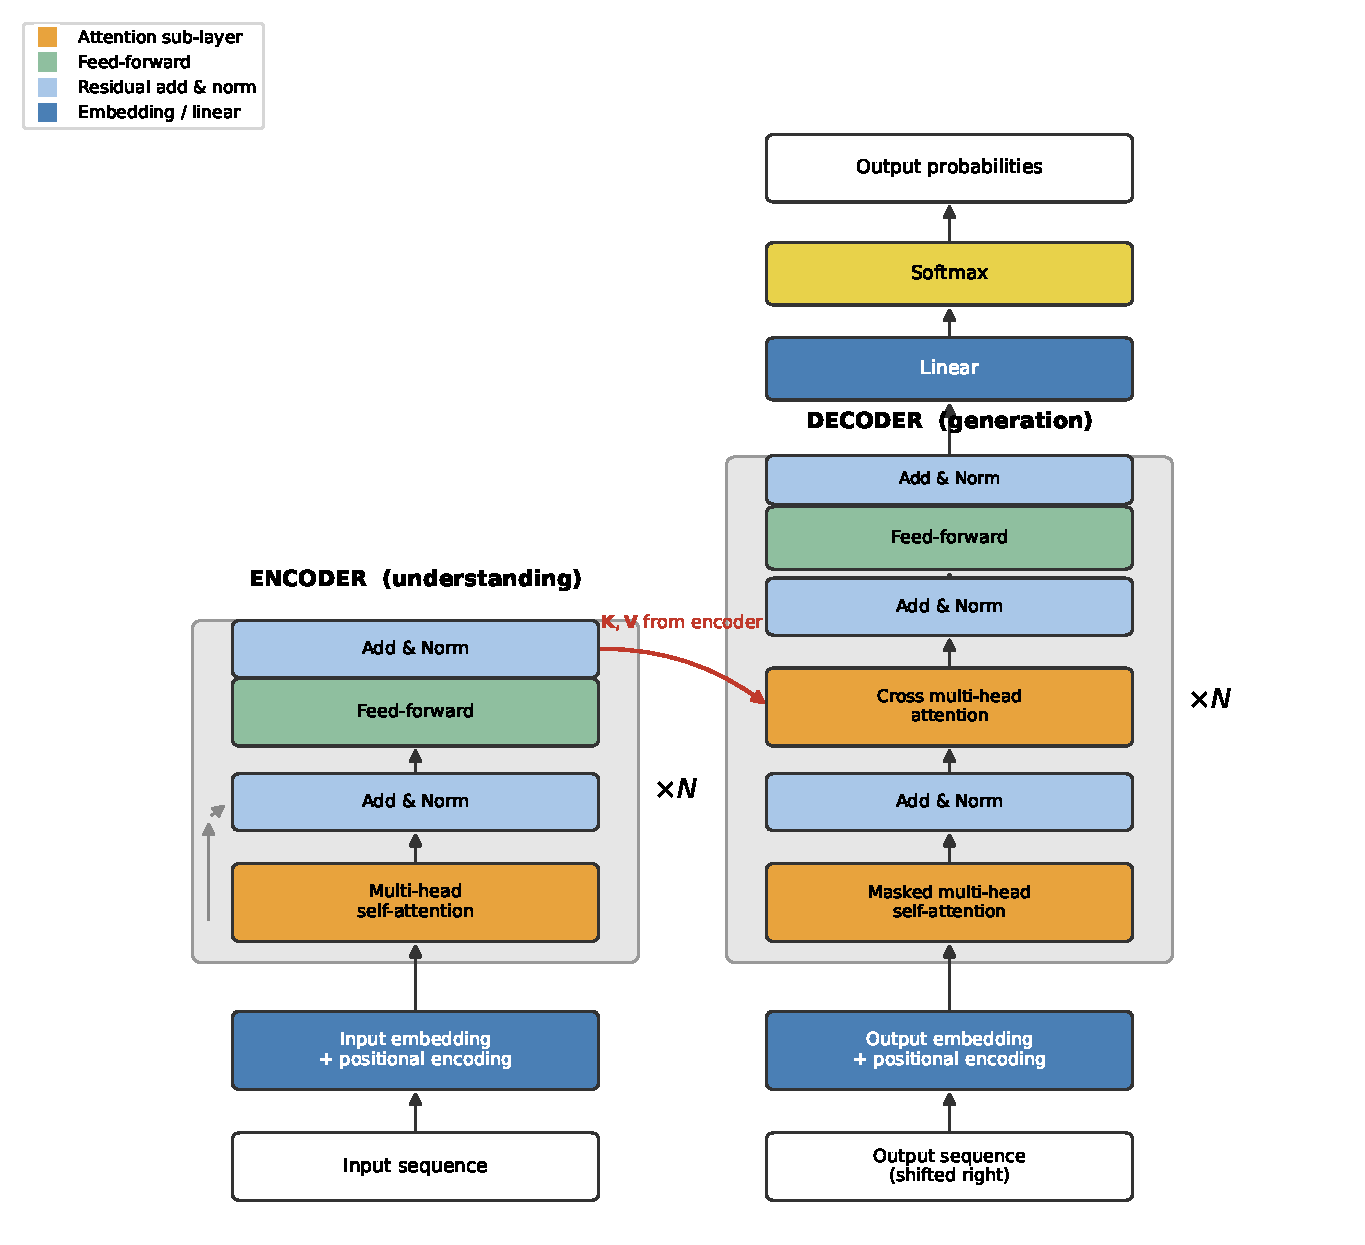
\includegraphics[width=0.7\linewidth]{files/figure_22_2_transfor-32e03fc756512304f5bc51ab8199c3b0.pdf}

FIGURE 22.2 makes the two data paths explicit. On the encoder side, each block applies multi-head self-attention followed by a feed-forward network, with every sub-layer wrapped in the residual add-and-normalise step of Equation (22.6), and the block is repeated N times. On the decoder side, an analogous stack inserts two extra pieces: a \textit{masked} self-attention, so that position $t$ cannot attend to tokens that come after it, and a \textit{cross-attention} sub-layer whose queries come from the decoder but whose keys and values come from the encoder output, which is how information flows from the input sequence to the generated one. A final linear projection followed by a softmax turns the top representation into a probability distribution over the vocabulary. The reader has met the words ``encoder'' and ``decoder'' before, in the autoencoder of Chapter 7, but the meaning here is different: the transformer's encoder and decoder do not compress and then reconstruct a single input, they map one sequence into another through attention.

We illustrate how self-attention resolves lexical ambiguity using a pre-trained transformer model.

\begin{verbatim}
from transformers import AutoTokenizer, AutoModel    # Hugging Face transformers
import torch

tokenizer = AutoTokenizer.from_pretrained('bert-base-uncased')
model = AutoModel.from_pretrained('bert-base-uncased',
                                  output_attentions=True)

sentences = [
    "The bank reported strong quarterly earnings.",   # Financial institution
    "We walked along the river bank at sunset.",      # River bank
]

for sent in sentences:
    inputs = tokenizer(sent, return_tensors='pt')
    with torch.no_grad():
        outputs = model(**inputs)
    # Extract embedding for "bank" token
    tokens = tokenizer.convert_ids_to_tokens(inputs['input_ids'][0])
    bank_idx = tokens.index('bank')
    embedding = outputs.last_hidden_state[0, bank_idx].numpy()
    print(f"'{sent}'")
    print(f"  'bank' at position {bank_idx}, "
          f"embedding norm: {np.linalg.norm(embedding):.3f}, "
          f"first 5 dims: {embedding[:5].round(3)}")
\end{verbatim}

\begin{verbatim}
'The bank reported strong quarterly earnings.'
  'bank' at position 2, embedding norm: 13.941, first 5 dims: [ 0.145 -0.421 -0.338  0.304  0.963]
'We walked along the river bank at sunset.'
  'bank' at position 6, embedding norm: 13.713, first 5 dims: [ 0.142 -0.66   0.029 -0.177 -0.21 ]
\end{verbatim}

The key observation is that the BERT embeddings for ``bank'' differ substantially between the two sentences, even though the word is identical. In the financial sentence, the embedding captures the meaning of ``bank'' as a financial institution (influenced by context words like ``earnings,'' ``quarterly,'' ``reported''). In the river sentence, the embedding reflects the geographical meaning (influenced by ``river,'' ``walked,'' ``sunset''). This is precisely the contextual understanding that static word embeddings (Chapter 21) cannot provide.

\begin{verbatim}
# Visualise attention pattern for the financial sentence
import matplotlib.pyplot as plt
inputs = tokenizer(sentences[0], return_tensors='pt')
with torch.no_grad():
    outputs = model(**inputs)

tokens = tokenizer.convert_ids_to_tokens(inputs['input_ids'][0])
attention = outputs.attentions[-1][0]                # Last layer, first head
attn_from_bank = attention[0, 2, :len(tokens)].numpy()  # Head 0, from "bank"

fig, ax = plt.subplots(figsize=(8, 4))
ax.bar(range(len(tokens)), attn_from_bank)
ax.set_xticks(range(len(tokens)))
ax.set_xticklabels(tokens, rotation=45, ha='right')
ax.set_ylabel('Attention weight')
ax.set_title("Attention from 'bank' to other tokens (last layer, head 0)")
plt.tight_layout()
plt.savefig('images/figure_22_1_bert_attention.png', dpi=140, bbox_inches='tight')
plt.show()
\end{verbatim}

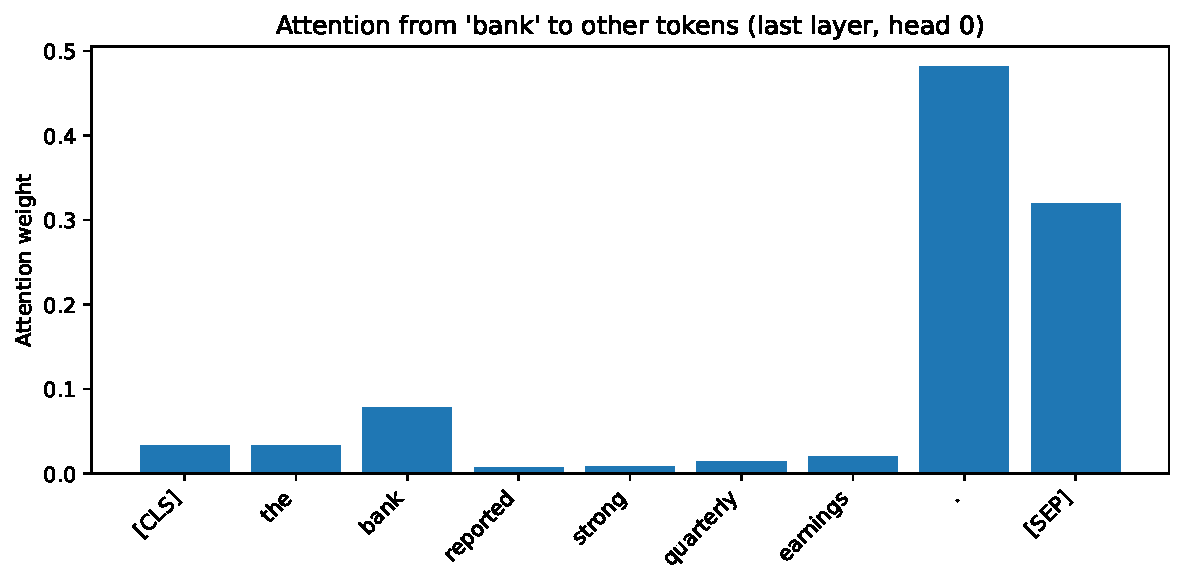
\includegraphics[width=0.7\linewidth]{files/figure_22_1_bert_att-ecea773b678058b459f5461fbc5aa46d.pdf}

As shown in FIGURE 22.1, the transformer concentrates attention from ``bank'' on the words ``earnings'' and ``reported,'' which disambiguate the financial meaning. This attention pattern demonstrates the mechanism by which transformers build contextual representations. As we discuss in Section 24.5, attention visualisation is also a useful interpretability tool for understanding what a model focuses on when making predictions.

\subsubsection{Architecture variants}

The original transformer of \cite{vaswani2017attention} contains both an encoder (which processes the input sequence) and a decoder (which generates the output sequence). Subsequent work has shown that using only the encoder or only the decoder yields powerful models for different tasks:

\begin{itemize}
\item \textbf{Encoder-only (BERT family).} The encoder processes the entire input sequence bidirectionally, meaning each token can attend to both left and right context. This is ideal for \textit{understanding} tasks: sentiment classification, named entity recognition, and textual similarity. BERT \citep{devlin2019bert} is the most prominent example.
\item \textbf{Decoder-only (GPT family).} The decoder processes tokens autoregressively, attending only to previous tokens (not future ones). This is ideal for \textit{generation} tasks: text completion, summarisation, and dialogue. GPT-2, GPT-3 \citep{brown2020language}, and subsequent models follow this paradigm.
\item \textbf{Encoder-decoder (T5, BART).} The full encoder-decoder architecture is used for \textit{sequence-to-sequence} tasks: translation, abstractive summarisation, and question answering. \cite{lewis2020bart} train BART as a denoising autoencoder in this family, and \cite{raffel2020exploring} showed that many NLP tasks can be framed in this text-to-text format.
\end{itemize}

The essential difference between the encoder-only and decoder-only families is not the depth of the stack but the \textit{attention mask} each one applies, illustrated in FIGURE 22.3.

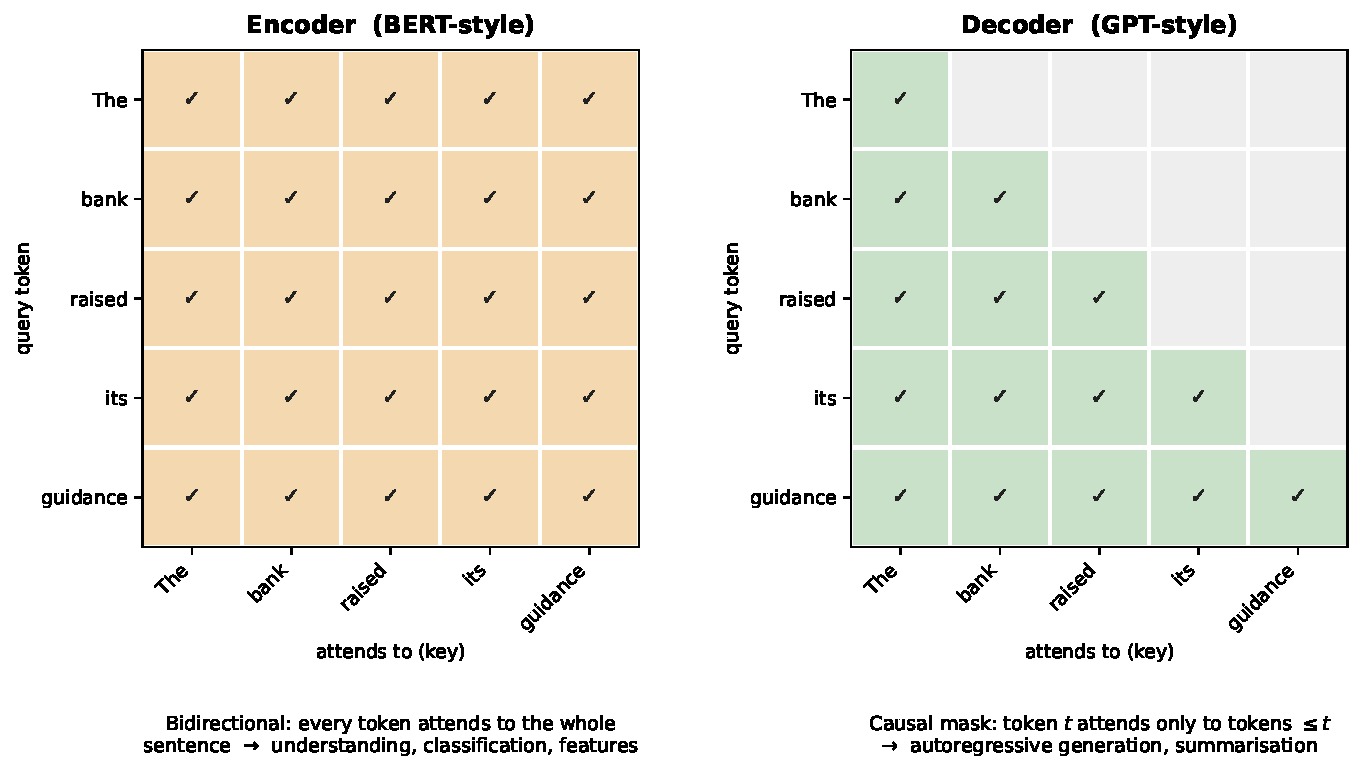
\includegraphics[width=0.7\linewidth]{files/figure_22_3_encoder_-b5ef1b82484dab5061b68639a352e06f.pdf}

The contrast in FIGURE 22.3 explains why the two families specialise as they do. Bidirectional attention lets an encoder condition each token's representation on the whole sentence, which is exactly what a sentiment classifier or a named-entity tagger needs, but it makes the model unusable for generation, since predicting the next word while already being allowed to see it is a degenerate task. The causal mask of the decoder removes that leakage, at the cost of context: each representation is built from the left only. For financial NLP, encoder-only models are most commonly used for classification and feature extraction, while decoder-only models (LLMs) are used for generation, summarisation, and zero-shot analysis. The encoder-only family is developed in the sections that follow; the decoder-only models that power large language models are the subject of Chapter 23.

\subsubsection{Transfer learning and fine-tuning}

Training a transformer from scratch requires enormous computational resources: BERT was pre-trained on 3.3 billion words (the entire English Wikipedia plus the BookCorpus) using 64 TPU chips for several days. Few financial practitioners have access to such resources. The solution is \textit{transfer learning}: pre-train a model on a large general-purpose corpus to learn the structure of language, then \textit{fine-tune} it on a small task-specific dataset to specialise it for the application of interest. \cite{howard2018ulmfit} established this pre-train-then-fine-tune paradigm for NLP text classification, showing that a language model pre-trained on general text could be adapted to a downstream task with only a modest labelled sample.

The pre-training phase teaches the model general linguistic knowledge: grammar, semantics, world knowledge, and reasoning patterns. The fine-tuning phase adapts this knowledge to a specific task (e.g., financial sentiment classification) using a much smaller labelled dataset, typically a few hundred to a few thousand examples. This approach works remarkably well because linguistic structure is largely shared across domains; what changes between general English and financial English is primarily vocabulary and domain-specific conventions.

\subsubsection{BERT and masked language modelling}

The value of bidirectional context had already been demonstrated by \cite{peters2018elmo}, whose ELMo model derived context-dependent word representations from a bidirectional LSTM language model; BERT brought this idea into the transformer. BERT (Bidirectional Encoder Representations from Transformers; \citep{devlin2019bert}) is pre-trained using two objectives:

\begin{enumerate}
\item \textbf{Masked language modelling (MLM).} Randomly select 15\% of the input tokens and train the model to predict them from context. In practice, of the selected positions, 80\% are replaced with a \texttt{[MASK]} token, 10\% with a random token, and 10\% are left unchanged, a scheme that reduces the mismatch between pre-training (which sees \texttt{[MASK]}) and fine-tuning (which does not). For example, given ``The [MASK] reported quarterly [MASK],'' the model must predict ``company'' and ``earnings.'' This forces the model to build rich bidirectional representations.
\item \textbf{Next sentence prediction (NSP).} Given two sentences concatenated with a \texttt{[SEP]} separator token, predict whether the second follows the first in the original text. This teaches the model about discourse coherence.
\end{enumerate}

Formally, let $\mathbf{x} = (x_1, \ldots, x_T)$ be an input token sequence and $\mathcal{M} \subset \{1, \ldots, T\}$ the random subset of masked positions (typically $|\mathcal{M}| = 0.15\, T$). The MLM objective is the masked negative log-likelihood,

\begin{equation}
\mathcal{L}_{\text{MLM}} = -\frac{1}{|\mathcal{M}|}\sum_{m \in \mathcal{M}} \log p_\theta(x_m \mid \mathbf{x}_{\setminus \mathcal{M}})
\tag{22.7}
\end{equation}

where $\mathbf{x}_{\setminus \mathcal{M}}$ denotes the input sequence with the positions in $\mathcal{M}$ replaced by a \texttt{[MASK]} token, and $\theta$ are the transformer parameters. The combined pre-training loss adds the binary next-sentence-prediction objective, $\mathcal{L}_{\text{BERT}} = \mathcal{L}_{\text{MLM}} + \mathcal{L}_{\text{NSP}}$. After pre-training, the model's internal representations (the output of the final transformer layer) serve as powerful features for downstream tasks. For classification, a simple linear layer is added on top of the \texttt{[CLS]} token embedding (a special token prepended to every input) and fine-tuned with labelled data.

\subsubsection{Finance-specific models}

General-purpose models like BERT sometimes struggle with financial text because of domain-specific vocabulary and conventions. Several finance-adapted models have been proposed:

\textbf{FinBERT} is in fact a family of three closely related models that are easily confused. The original \cite{araci2019finbert} version further pre-trained BERT on Reuters TRC2-financial news and fine-tuned it on the Financial PhraseBank sentiment benchmark. \cite{yang2020finbert} released a separate FinBERT trained from scratch on a much larger 4.9-billion-token corpus of corporate reports, earnings-call transcripts, and analyst reports, which has become the de facto open-source FinBERT in practitioner pipelines. \cite{huang2023finbert} then introduced a third FinBERT released alongside their \textit{Contemporary Accounting Research} paper, pre-trained on a still broader financial corpus and benchmarked on a wider battery of finance NLP tasks. All three significantly outperform general-purpose BERT and dictionary methods on financial sentiment benchmarks, and the differences between them matter mostly when reproducing prior numbers: the choice of pre-training corpus drives most of the residual gap.

\textbf{ClimateBERT} \citep{webersinke2022climatebert} is adapted for climate-related text, trained on climate disclosures, IPCC reports, and sustainability publications. It enables automated analysis of climate risk in corporate filings, a task of growing importance for ESG-oriented investors.

Domain adaptation is not confined to encoder models. \cite{wu2023bloomberggpt} train BloombergGPT, a decoder-only large language model, from scratch on a corpus that mixes financial and general-purpose text, producing a finance-specialised counterpart to the general generative models taken up in Chapter 23.

A parallel strand of research applies transformer architectures specifically to earnings-call transcripts, which pose a distinctive challenge because of their length (often thousands of tokens) and mixed register (formal prepared remarks followed by unscripted Q\&A). \cite{yang2020html} address this with HTML (Hierarchical Transformer-based Multi-task Learning), a model that segments a transcript into utterance-level blocks, applies a local transformer within each block, and then applies a second transformer across blocks to capture discourse-level structure. Trained jointly to predict both short-term volatility and price direction, HTML outperformed flat BERT and RNN baselines on earnings-call benchmarks, and it established the hierarchical transformer as the canonical architecture for long financial documents. The fact that the academic transcript literature \citep{yang2020html} and the practitioner transcript literature surveyed in Chapter 20 converge on the same genre of text underscores the importance of earnings calls as a signal source.

The common thread is \textit{domain adaptation}: starting from a general pre-trained model and further training on domain-specific text. This approach combines the linguistic knowledge from general pre-training with the specialised vocabulary and conventions of finance. It is worth emphasising a division of labour that the architecture motivates: these contextual encoder models excel at \textit{classification} tasks (sentiment, topic, entity type), where a single label is attached to the full input. For \textit{similarity} tasks across pairs of sentences or documents (peer-group construction, filing-change detection, cross-asset analogies), the sentence-transformer family of Section 21.4 is the more appropriate tool, because its contrastive training objective calibrates cosine distances in a way that the masked-language-modelling objective of standard BERT does not.

We apply FinBERT to the same six KO-flavoured sentences used in the Loughran-McDonald demonstration of Section 20.4 and compare its classifications directly against the dictionary approach.

\begin{verbatim}
from transformers import pipeline                    # High-level inference API

finbert = pipeline(
    'sentiment-analysis',
    model='ProsusAI/finbert',                        # Pre-trained FinBERT
    tokenizer='ProsusAI/finbert'
)

test_sentences = [                                   # the same six sentences scored in Section 20.4
    "Revenue growth was strong driven by innovation across our beverage portfolio.",
    "The softness in price mix was attributed to unfavorable category mix and constrained production capacity.",
    "Operating losses did not materialize, and margins held firm.",
    "Free cash flow improved and management sees favorable conditions for the remainder of the year.",
    "Adverse macroeconomic conditions and persistent inflation pose a risk to near-term consumer demand.",
    "The firm achieved outstanding results with superior margin expansion in North America.",
]

results = finbert(test_sentences)
for i, (sent, res) in enumerate(zip(test_sentences, results)):
    print(f"Doc {i}: {res['label']:>8s} ({res['score']:.3f})  {sent[:55]}...")
\end{verbatim}

\begin{verbatim}
Doc 0: positive (0.954)  Revenue growth was strong driven by innovation across o...
Doc 1: negative (0.950)  The softness in price mix was attributed to unfavorable...
Doc 2: positive (0.893)  Operating losses did not materialize, and margins held ...
Doc 3: positive (0.956)  Free cash flow improved and management sees favorable c...
Doc 4: negative (0.884)  Adverse macroeconomic conditions and persistent inflati...
Doc 5: positive (0.958)  The firm achieved outstanding results with superior mar...
\end{verbatim}

The contrast with the dictionary approach (Section 20.4) is striking. FinBERT correctly classifies Doc 2 (``Operating losses did not materialize, and margins held firm'') as positive with 89.3\% confidence, whereas the Loughran-McDonald dictionary scored it as -1.00. The model's contextual understanding of negation is its key advantage: it processes ``losses did not materialize'' as a single negated expression rather than counting ``losses'' in isolation.

\begin{verbatim}
# Compare FinBERT vs. dictionary on the same sentences
import pandas as pd
dict_scores = [1.0, -1.0, -1.0, 1.0, -1.0, 1.0]      # Loughran-McDonald net tone from Section 20.4
finbert_scores = [1.0 if r['label'] == 'positive'
                  else -1.0 if r['label'] == 'negative'
                  else 0.0 for r in results]

comparison = pd.DataFrame({
    'Dictionary': dict_scores,
    'FinBERT': finbert_scores,
    'Agree': [d * f > 0 for d, f in zip(dict_scores, finbert_scores)]
}, index=[f'Doc {i}' for i in range(len(dict_scores))])
print(comparison.to_string())
\end{verbatim}

\begin{verbatim}
Dictionary  FinBERT  Agree
Doc 0         1.0      1.0   True
Doc 1        -1.0     -1.0   True
Doc 2        -1.0      1.0  False
Doc 3         1.0      1.0   True
Doc 4        -1.0     -1.0   True
Doc 5         1.0      1.0   True
\end{verbatim}

The two methods agree on five of six sentences. The disagreement on Doc 2 highlights the negation-handling advantage of transformer-based models. In a large-scale evaluation this type of error correction accumulates, though the resulting lift over a well-tuned lexicon is typically modest.

\subsubsection{When to use FinBERT (and when not to)}

The practical gains of contextual representations are largest precisely for the failure modes catalogued in Section 20.4: negation, conditional language, and context-dependent polarity, cases in which the sentiment carried by a word depends on the words around it. Because FinBERT encodes each token in the context of the whole sentence rather than scoring it in isolation, it resolves many of the cases that a fixed lexicon systematically mishandles, and on standard financial-sentiment benchmarks it is usually the more accurate of the two. That advantage is genuine, but it is bounded, and it is worth being precise about where it stops.

Fine-tuned models are not a panacea. They require labelled training data, which is expensive to create for finance; they can be sensitive to the distribution of that data, so a model fine-tuned on news may underperform on earnings calls; and they are computationally heavier than dictionary lookups. For text that is relatively formulaic (standardised filings, for instance) and whose vocabulary is stable, dictionary methods remain a cost-effective baseline, a point the survey of textual analysis in accounting and finance by \cite{loughran2016textual} makes at length. More pointedly, FinBERT is no longer the frontier it once was: \cite{fatouros2023chatgpt} report that a general-purpose large language model (ChatGPT), simply prompted, outperforms FinBERT on financial-sentiment classification by roughly a third and correlates more strongly with subsequent returns, so the domain-specific fine-tune no longer dominates a general model that can be steered with a well-written prompt. A second and more unsettling line of criticism concerns robustness. \cite{leippold2023sentiment} shows that financial sentiment scores can be adversarially manipulated: paraphrasing a sentence with a language model flips a keyword classifier's verdict in close to 99\% of negative cases, and although context-aware encoders looked comparatively resistant in that study, \cite{turetken2026battle} go on to show that the transformer sentiment models themselves, FinBERT included, can be fooled by targeted attacks. The concern is not merely academic, since firms increasingly craft disclosures in the knowledge that machines will read them, so any deployed sentiment model operates in a setting where the very text it scores is partly written to move the score. The reasonable conclusion is not that FinBERT should be avoided, but that its output is one noisy, potentially gameable signal among several, best combined with dictionary and market-based measures rather than trusted on its own.

\subsubsection{Coding exercises}

\begin{enumerate}
\item Load a pre-trained FinBERT model with the \texttt{transformers} library and extract the
\texttt{[CLS]} token embedding for each of the six example sentences of Section 22.7.
Compute the pairwise cosine-similarity matrix of the embeddings, identify the pair
of sentences the model considers most similar, and comment on whether the grouping
reflects the topic of the sentences or their sentiment.
\end{enumerate}

\subsubsection{References}